\section{De l'algèbre aux composants}\label{sec:contrib:astronef:architecture}
Dans cette section, nous détaillons les éléments d'architectures que nous avons mis en œuvre pour permettre à une requête Astral d'être instanciée en un processus de traitement. Nous abordons premièrement les principes architecturaux utilisés. Ensuite, nous détaillons les différents composants utilisés dans Astronef. Enfin, nous présentons notre méthode extensible de construction de plan par l'utilisation d'un système de règles.
\subsection{Architecture}
Avant de détailler l'architecture de notre système de traitement de requêtes continues, nous allons d'abord présenter le paradigme architectural dans lequel nous allons mettre en œuvre Astronef. Nous présentons premièrement et brièvement les architectures à services. Puis, nous détaillons les principes des architectures à composants orientés services que nous utilisons par la suite.
\subsubsection{Architecture à service}
Les architectures à services permettent aux applications d'être assemblés sous forme de blocs réutilisables étant des \textit{services}. Un \textit{service} est définit par une spécification (ou \textit{description}, ou \textit{contrat}), qui décrit sa syntaxe, son comportement, sa sémantique ainsi que sa dépendance aux autres services. Dans les architectures à service, les services interagissent via un patron récurrent d'interaction (fig~\ref{fig:contrib:astronef:services}). 
\begin{figure}[ht]
    \centering
    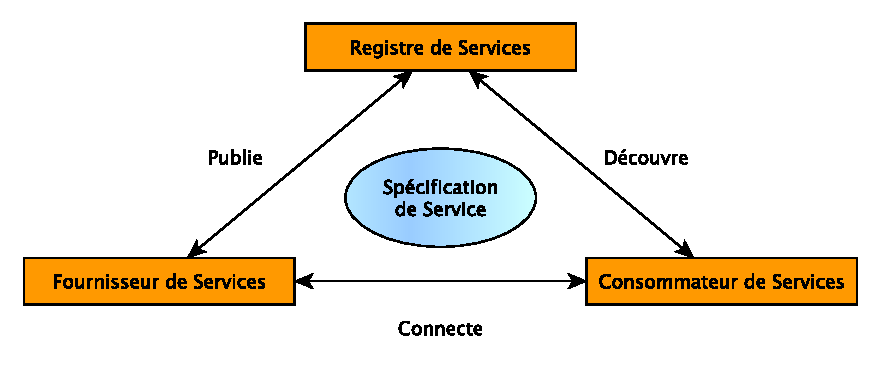
\includegraphics[width=0.7\textwidth]{contrib-astronef-services}
    \caption{Patron d'interaction de service}\label{fig:contrib:astronef:services}
\end{figure}
Un fournisseur de service va publier sa spécification à un registre. Un consommateur de service découvre le service fournit par une requête sur le registre. Enfin, le consommateur et le fournisseur se connectent. Le point clé de cette architecture étant que cette résolution est faite au \textit{runtime}.

\subsubsection{Architecture à composants orientés services}
Le modèle d'architecture à composants orientés services~\cite{Cervantes:servicecomponent} permet la mise en œuvre d'applications à base de services dans le paradigme de la programmation par composants. Le principe étant de séparer les mécanismes des architectures à services du code implémentant le comportement du service fournit. Ainsi, voici les principes d'un tel modèle :
\begin{itemize}
    \item Un service est une fonctionnalité fournie.
    \item Un service est caractérisé par sa spécification.
    \item Les composants implémentent des spécifications de services, qui peuvent eux-mêmes dépendre, du fait de leurs implémentations, d'autres services.
    \item Les patrons d'interactions de services sont utilisés pour résoudre les dépendances de services au \textit{runtime}.
    \item Les compositions sont décrites en terme de spécifications de services.
    \item Tout composant peut se substituer par un autre si les spécifications de services sont identiques.
\end{itemize}
Nous mêlons donc dans un même modèle, les idées de composants et de services. De plus, en s'inspirant des modèles récents tels que Fractal~\cite{Bruneton:fractal}, chaque composant possède un ensemble de propriétés (ou attributs) configurables. Nous obtenons aussi le pouvoir d'instancier (grâce aux fabriques) des composants à partir de configurations.

\begin{figure}[ht]
    \centering
    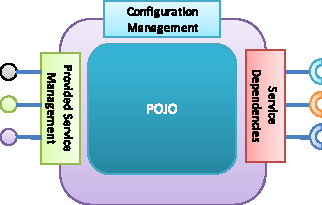
\includegraphics[width=0.5\textwidth]{contrib-astronef-ipojo}
    \caption{Un composant iPojo}\label{fig:contrib:astronef:ipojo}
\end{figure}
La figure~\ref{fig:contrib:astronef:ipojo} représente un composant dans l'implémentation \textit{iPojo}~\cite{Escoffier:ipojo}. Le principe étant que le code du composant (le \textit{POJO}, \textit{Plain Old Java Object}) est embarqué dans un conténaire auxquels seront accrochés des gestionnaires. Les trois couramment utilisés sont les gestionnaires de dépendances, de production de service, et de configuration. Ainsi, un composant pourra s'exposer sur un registre, tout en dépendant d'autres services et en supportant le fait d'être configurable.

\subsection{Les différents composants et services}
L'architecture d'Astronef est entièrement dirigé par ces approches. De multiples composants sont ainsi créés et instantiables, pour former une requête. Afin de pouvoir exécuter les requêtes, nous définissons trois services centraux :
\begin{itemize}
	\item[\textbf{Les \textit{EventProcessor}}] : Ces services ont deux primitives, l'une exécute une tâche quelconque, l'autre indique les autres \textit{EventProcessors} dont il dépend.
	\item[\textbf{Le \textit{Scheduler}}] : Ce service permet la planification. Ses primitives permettent aux différents \textit{EventProcessor} d'exprimer leur volonté de s'exécuter. Ce service devra mettre en ordre ces demandes en fonction des dépendances exprimés.
	\item[\textbf{Le \textit{QueryRuntime}}] : Ce service permet d'exécuter une requête. Il est lié à un \textit{Scheduler}, et utilise la primitive \textit{next} de celui-ci pour connaître la prochaine tâche qu'il faudra exécuter.
\end{itemize}

Nous adoptons ainsi l'approche émise par~\cite{Carney:scheduling} pour gérer l'ordonnancement des événements. Maintenant que nous avons vu les différents services nécessaire à l'exécution. Nous avons plusieurs types de composants que nous pourrons instantier :
\begin{itemize}
	\item[\textbf{Les entités}] : Fournissent les services nécessaires pour manipuler un flux ou une relation. Ces entités servent de résultats intermédiaires (ou de tampons). De plus, ils permettent un service de notification. En cas de changement, les \textit{EventProcessor} abonnés seront notifiés. Ainsi, ces composants nécessitent un \textit{Scheduler} pour demander l'exécution de leurs abonnés.
	\item[\textbf{Les sources}] : Une source nécessite une entité en lecture, dont elle manipulera le contenu pour la remplir. Ce composant pourra nécessiter le \textit{Scheduler} pour, entre autres, notifier la fin de son envoi et donc la fin de la requête.
	\item[\textbf{Les opérateurs}] : Nécessitent $n$ entités en lecture, et une autre particulière en écriture. Ce composant doit fournir le service \textit{EventProcessor}. Les implémentations des opérateurs bloquants pourront faire appel au \textit{Scheduler} pour planifier des exécutions ponctuelles.
	\item[\textbf{Les puits}] : Nécessitent une entité en lecture. Ce composant fournit le service \textit{EventProcessor} et doit être non-bloquant (donc seulement s'abonner à son entité en lecture).
\end{itemize}

Ainsi pour créer une requête : l'utilisateur doit fournir un ou plusieurs composants sources et un composant puit. Par la suite, il demande à Astronef de lui instantier ses sources et son puit en configurant les composants selon sa volonté. Enfin, il spécifie l'expression algébrique liant les sources au puit.

\subsubsection{De l'importance de la réutilisation}
Le fait d'abstraire l'architecture d'\textit{Astronef} permet une grande flexibilité architecturale. Tout d'abord, pour chaque composant, le fait de pouvoir le configurer tout en gérant son cycle de vie permet de réutiliser le même module pour plusieurs usages. Par exemple, supposons l'existance d'une source capable de récupérer une information périodiquement sur un protocole donné. Cette source pourra être utilisé pour plusieurs requêtes sous différentes instances en ayant plusieurs configurations.

Mais cette abstraction sous forme de services permet surtout la substitution. En effet, nous pouvons remplacer n'importe quel composant du moment qu'il supporte le même service. Nous utilisons ce principe pour sélectionner les meilleurs composants pour remplir le plus efficacement leurs rôles. De plus, l'utilisateur peut apporter ses propres implémentations pour étendre les capacités de l'intergiciel.

\subsection{Construction du plan par règles}
Nous définissons un plan de requête comme un ensemble de composants déployés pour répondre à la requête de l'utilisateur. Nous souhaitons avant tout que l'utilisateur n'ai pas à intervenir lors de cette construction. De son point de vue, il ne doit écrire que l'expression algébrique de sa requête et il doit être garanti d'une mise en œuvre efficace.

Pour atteindre ce but, nous avons choisi de mettre en place un moteur de règle. Le principe étant que nous partons de l'expression algébrique, puis nous itérons suivant plusieurs schéma d'inférences jusqu'à obtenir un plan de requête. Nous remarquons plusieurs avantage à une telle approche :
\begin{itemize}
	\item Intégration naturelle des connaissances. L'algèbre est pleine de propriété et de théorèmes. Il est nécessaire de pouvoir les exprimer dans un langage déclaratif pour les exploiter et pour en rajouter le plus possible.
	\item Expression de la sémantique des composants par l'algèbre. Comme il est nécessaire d'associer des composants logiciels à la sémantique d'Astral, il est nécessaire de spécifier à quelle opération chaque composant (et chaque paramètre de configuration) répond. Cela permet une clarification des sémantiques d'exécution.
	\item Extensibilité très forte. En considérant que l'ajout de nouveaux composants peut se faire via l'ajout de nouvelles règles, il devient aisé d'étendre le système pour permettre des opérateurs, ou des optimisations qui n'étaient pas prévues.
\end{itemize}

Afin de mettre en œuvre cet ensemble de règle pour obtenir un plan de requête efficace, nous faisons une analogie avec les systèmes de gestions de base de données. Comme présenté dans la section~\ref{sec:rw:sgfd:optim}, l'optimisation est découpé en deux parties : l'optimisation logique, et l'optimisation physique. Nous réutiliserons cette approche qui a fait ses preuves au fur et à mesure des années. Nous restructurerons donc la structure de l'expression algébrique dans la section~\ref{sec:contrib:astronef:logique} pour qu'elle soit plus optimisé. Ensuite, nous sélectionnerons les meilleurs composants et les meilleures configurations pour mettre en œuvre cette nouvelle expression, dans la section~\ref{sec:contrib:astronef:physique}.

Nous utilisons un moteur capable d'exécuter du Prolog~\footnote{En réalité, le langage utilisé (PROVA~\cite{Kozlenkov:prova}) est un dérivé de Prolog mieux adapté à l'intégration avec Java. Mais le principe reste tout à fait similaire.}, langage de programmation logique, pour appliquer nos règles. Avant de détailler l'ensemble de ces règles, nous présentons d'abord la structure d'une expression. Toute expression étant structuré sous forme d'arbre, il est possible de représenter une requête avec des nœuds de la forme\footnote{L'utilisation d'objets de propriétés fait partie du langage PROVA, mais cela reste formalisable en Prolog standard avec une liste d'éléments [clé,valeur].} :
\begin{center} [$\underbrace{A}_{\textrm{Nature du nœud}}$, $\underbrace{B}_{\textrm{Ensemble de propriétés}}$, $\underbrace{C}_{\textrm{Liste de nœuds fils}}$] \end{center}
\begin{example}
	Soit $R$ une source déclaré dans le système, nous souhaitons exécuter la requête $\sigma_{id=1} R$. Alors l'expression de cette requête est la suivante :
	\begin{lstlisting}
[sigma,	{"condition":"id=1"}, [
	[source, {id:"R"}, []]
]]
	\end{lstlisting}
\end{example}
Nous remarquons que cette syntaxe est très similaire au \textit{XML}, c'est pour cela que ce langage est celui utilisé en pratique pour spécifier des requêtes dans le prototype. Il est ensuite traduit en expression utilisable en Prolog. L'ensemble des nœuds possibles corresponds aux différents opérateurs de l'algèbre. Nous ne détaillerons pas ceci dans ce manuscrit. Le lecteur pourra consulter le manuel sur la page web suivante \url{http://code.google.com/p/astral/wiki/XMLSyntax} pour trouver les expressions exactes supportées.